%  LaTeX support: latex@mdpi.com 
%  For support, please attach all files needed for compiling as well as the log file, and specify your operating system, LaTeX version, and LaTeX editor.

%=================================================================
\documentclass[idr,communication,submit,oneauthor,pdftex]{Definitions/mdpi}

% For posting an early version of this manuscript as a preprint, you may use "preprints" as the journal and change "submit" to "accept". The document class line would be, e.g., \documentclass[preprints,article,accept,moreauthors,pdftex]{mdpi}. This is especially recommended for submission to arXiv, where line numbers should be removed before posting. For preprints.org, the editorial staff will make this change immediately prior to posting.

%--------------------
% Class Options:
%--------------------
%----------
% journal
%----------
% Choose between the following MDPI journals:
% acoustics, actuators, addictions, admsci, adolescents, aerospace, agriculture, agriengineering, agronomy, ai, algorithms, allergies, analytica, animals, antibiotics, antibodies, antioxidants, appliedchem, applmech, applmicrobiol, applnano, applsci, arts, asi, atmosphere, atoms, audiolres, automation, axioms, batteries, bdcc, behavsci, beverages, biochem, bioengineering, biologics, biology, biomechanics, biomedicines, biomedinformatics, biomimetics, biomolecules, biophysica, biosensors, biotech, birds, bloods, brainsci, buildings, businesses, cancers, carbon, cardiogenetics, catalysts, cells, ceramics, challenges, chemengineering, chemistry, chemosensors, chemproc, children, civileng, cleantechnol, climate, clinpract, clockssleep, cmd, coatings, colloids, compounds, computation, computers, condensedmatter, conservation, constrmater, cosmetics, crops, cryptography, crystals, curroncol, cyber, dairy, data, dentistry, dermato, dermatopathology, designs, diabetology, diagnostics, digital, disabilities, diseases, diversity, dna, drones, dynamics, earth, ebj, ecologies, econometrics, economies, education, ejihpe, electricity, electrochem, electronicmat, electronics, encyclopedia, endocrines, energies, eng, engproc, entropy, environments, environsciproc, epidemiologia, epigenomes, fermentation, fibers, fire, fishes, fluids, foods, forecasting, forensicsci, forests, fractalfract, fuels, futureinternet, futuretransp, futurepharmacol, futurephys, galaxies, games, gases, gastroent, gastrointestdisord, gels, genealogy, genes, geographies, geohazards, geomatics, geosciences, geotechnics, geriatrics, hazardousmatters, healthcare, hearts, hemato, heritage, highthroughput, histories, horticulturae, humanities, hydrogen, hydrology, hygiene, idr, ijerph, ijfs, ijgi, ijms, ijns, ijtm, ijtpp, immuno, informatics, information, infrastructures, inorganics, insects, instruments, inventions, iot, j, jcdd, jcm, jcp, jcs, jdb, jfb, jfmk, jimaging, jintelligence, jlpea, jmmp, jmp, jmse, jne, jnt, jof, joitmc, jor, journalmedia, jox, jpm, jrfm, jsan, jtaer, jzbg, kidney, land, languages, laws, life, liquids, literature, livers, logistics, lubricants, machines, macromol, magnetism, magnetochemistry, make, marinedrugs, materials, materproc, mathematics, mca, measurements, medicina, medicines, medsci, membranes, metabolites, metals, metrology, micro, microarrays, microbiolres, micromachines, microorganisms, minerals, mining, modelling, molbank, molecules, mps, mti, nanoenergyadv, nanomanufacturing, nanomaterials, ncrna, network, neuroglia, neurolint, neurosci, nitrogen, notspecified, nri, nursrep, nutrients, obesities, oceans, ohbm, onco, oncopathology, optics, oral, organics, osteology, oxygen, parasites, parasitologia, particles, pathogens, pathophysiology, pediatrrep, pharmaceuticals, pharmaceutics, pharmacy, philosophies, photochem, photonics, physchem, physics, physiolsci, plants, plasma, pollutants, polymers, polysaccharides, proceedings, processes, prosthesis, proteomes, psych, psychiatryint, publications, quantumrep, quaternary, qubs, radiation, reactions, recycling, regeneration, religions, remotesensing, reports, reprodmed, resources, risks, robotics, safety, sci, scipharm, sensors, separations, sexes, signals, sinusitis, smartcities, sna, societies, socsci, soilsystems, solids, sports, standards, stats, stresses, surfaces, surgeries, suschem, sustainability, symmetry, systems, taxonomy, technologies, telecom, textiles, thermo, tourismhosp, toxics, toxins, transplantology, traumas, tropicalmed, universe, urbansci, uro, vaccines, vehicles, vetsci, vibration, viruses, vision, water, wevj, women, world 

%---------
% article
%---------
% The default type of manuscript is "article", but can be replaced by: 
% abstract, addendum, article, book, bookreview, briefreport, casereport, comment, commentary, communication, conferenceproceedings, correction, conferencereport, entry, expressionofconcern, extendedabstract, datadescriptor, editorial, essay, erratum, hypothesis, interestingimage, obituary, opinion, projectreport, reply, retraction, review, perspective, protocol, shortnote, studyprotocol, systematicreview, supfile, technicalnote, viewpoint, guidelines, registeredreport, tutorial
% supfile = supplementary materials

%----------
% submit
%----------
% The class option "submit" will be changed to "accept" by the Editorial Office when the paper is accepted. This will only make changes to the frontpage (e.g., the logo of the journal will get visible), the headings, and the copyright information. Also, line numbering will be removed. Journal info and pagination for accepted papers will also be assigned by the Editorial Office.

%------------------
% moreauthors
%------------------
% If there is only one author the class option oneauthor should be used. Otherwise use the class option moreauthors.

%---------
% pdftex
%---------
% The option pdftex is for use with pdfLaTeX. If eps figures are used, remove the option pdftex and use LaTeX and dvi2pdf.

%=================================================================
% MDPI internal commands
\firstpage{1} 
\makeatletter 
\setcounter{page}{\@firstpage} 
\makeatother
\pubvolume{1}
\issuenum{1}
\articlenumber{0}
\pubyear{2021}
\copyrightyear{2020}
%\externaleditor{Academic Editor: Firstname Lastname} % For journal Automation, please change Academic Editor to "Communicated by"
\datereceived{} 
\dateaccepted{} 
\datepublished{} 
\hreflink{https://doi.org/} % If needed use \linebreak
%------------------------------------------------------------------
% The following line should be uncommented if the LaTeX file is uploaded to arXiv.org
%\pdfoutput=1

%=================================================================
% Add packages and commands here. The following packages are loaded in our class file: fontenc, inputenc, calc, indentfirst, fancyhdr, graphicx, epstopdf, lastpage, ifthen, lineno, float, amsmath, setspace, enumitem, mathpazo, booktabs, titlesec, etoolbox, tabto, xcolor, soul, multirow, microtype, tikz, totcount, changepage, paracol, attrib, upgreek, cleveref, amsthm, hyphenat, natbib, hyperref, footmisc, url, geometry, newfloat, caption

%=================================================================
%% Please use the following mathematics environments: Theorem, Lemma, Corollary, Proposition, Characterization, Property, Problem, Example, ExamplesandDefinitions, Hypothesis, Remark, Definition, Notation, Assumption
%% For proofs, please use the proof environment (the amsthm package is loaded by the MDPI class).

%=================================================================
% Full title of the paper (Capitalized)
\Title{VAERS data reveals no increased risk of neuroautoimmune adverse events from COVID-19 vaccines}

% MDPI internal command: Title for citation in the left column
\TitleCitation{VAERS data reveals no increased risk of neuroautoimmune adverse events from COVID-19 vaccines}

% Author Orchid ID: enter ID or remove command
\newcommand{\orcidauthorA}{0000-0003-3131-0864} % Add \orcidA{} behind the author's name

% Authors, for the paper (add full first names)
\Author{Chris von Csefalvay$^{1}$\orcidA{}}

% MDPI internal command: Authors, for metadata in PDF
\AuthorNames{Chris von Csefalvay}

% MDPI internal command: Authors, for citation in the left column
\AuthorCitation{von Csefalvay, C.}
% If this is a Chicago style journal: Lastname, Firstname, Firstname Lastname, and Firstname Lastname.

% Affiliations / Addresses (Add [1] after \address if there is only one affiliation.)
\address{%
$^{1}$ \quad Starschema Inc., Arlington, VA; csefalvayk@starschema.net}

% Contact information of the corresponding author
\corres{Correspondence: csefalvayk@starschema.net}


% Abstract (Do not insert blank lines, i.e. \\)
\abstract{Neuroautoimmune disorders, such as multiple sclerosis and Guillain-Barre syndrome, have been documented in
relation to various vaccines in the past. This paper uses passive reporting information from the CDC/FDA's VAERS
system to analyse whether neuroautoimmune presentations are reported at a relatively higher or lower rate, vis-a-vis
other adverse effects, for COVID-19 vaccines than for other vaccines. Through computing the reporting odds ratios for
a range of symptoms and comparator vaccines, a clear indication in favour of the safety of COVID-19 vaccines
emerges, with reports of neuroautoimmune adverse events in relation to other adverse events being over 70\% less
likely for COVID-19 than for comparator vaccines ($ROR: 0.292$, $p < 0.0001$). In comparison with other vaccines given
as part of routine care in adulthood, COVID-19 vaccines have the lowest reporting odds ratio of neuroautoimmune
adverse effects (median $ROR$: $0.246$).}

% Keywords
\keyword{Neuroautoimmune disorders, demyelinating disorders, vaccine safety, pharmacovigilance, COVID-19 vaccines}

% The fields PACS, MSC, and JEL may be left empty or commented out if not applicable
%\PACS{J0101}
%\MSC{}
%\JEL{}

\begin{document}
%%%%%%%%%%%%%%%%%%%%%%%%%%%%%%%%%%%%%%%%%%

\section{Introduction}

The global drive to curb the spread of COVID-19 through a concerted vaccination effort is undoubtedly one of the most
ambitious public health projects ever undertaken. At the time of writing, only a little over six months after the FDA
granted EUAs to the first two of eventually three SARS-CoV-2 vaccines in early December, over 43\% of the U.S.
population has been fully vaccinated (i.e. two doses of a two-dose vaccine or a single dose of a one-dose vaccine). For
comparison, during the severe 2017-18 flu season, only 37.1\% of adults were vaccinated.\cite{centers2018estimates}

To safeguard this unprecedented accomplishment, it is crucial to exercise close surveillance of potential adverse
events (AEFIs). At least partially owing to the fact that the Moderna and Pfizer/BioNTech vaccines are first-in-man
applications of mRNA vaccine technology at scale, a significant number of eligible individuals have refused to be
vaccinated.\cite{dror2020vaccine,robertson2021predictors,troiano2021vaccine} The fear of adverse effects, both short and
long term, is undoubtedly a driving factor that fuels these apprehensions and eventually results in an overall
reluctance to be vaccinated. Among mid- to long-term AEFIs, neurological AEFIs hold a particular place, as is evident
from studies on reasons behind vaccine refusal.\cite{berry2021lessons} The bitter past experience with Guillain-Barre
syndrome (GBS) as a side effect of certain influenza vaccines, esp. the much publicised association between 1976-77
A/New Jersey/8/76 influenza vaccines and GBS, is still within living memory.\cite{haber2004guillain} Similarly
well-known is the association between the recombinant hepatitis B vaccine and multiple
sclerosis.\cite{hernan2004recombinant} In addition, the  emergence of various theories about a purported (and
disproven) causal mechanism between autism spectrum disorders and vaccinations that hypothesises an autoimmune
pathogenetic process has created a persistent point of rhetoric that erroneously portrays vaccines as inevitably
likely to cause neuroautoimmunity.\cite{poland2001understanding} Given the often devastating economic, social,
psychological and QoL impact of neuroautoimmune diseases,\cite{marck2020predictors,miller2006health,patwardhan2005cost}
some degree of apprehension appears natural.

It is beyond the scope of this paper to outline the range of potential pathophysiological mechanisms that may underlie
autoimmunity, including neuroautoimmunity, following a vaccination (for such a review, see Wraith et al.
(2003)\cite{wraith2003vaccination}). Rather, we seek to identify evidence regarding the safety of COVID-19 vaccines
approved in the United States (Pfizer/BioNTech, Moderna and Johnson \& Johnson) with regard to neuroautoimmune AEFIs
through an analysis of VAERS.

As with all studies leveraging VAERS, its limitations must be read in conjunction with results derived from VAERS data. Like
all passive pharmacovigilance systems, it relies on reporting. Under the terms of the EUAs granted to each of the three
vaccine manufacturers, COVID-19 vaccination providers must report any

\begin{itemize}
\item	vaccine administration errors (regardless of consequence);
\item	serious AEFI (regardless of causal attribution), incl. any AEFI resulting in inpatient admission, long-term
disability or death; and
\item	instances of multi-system inflammatory syndrome,
\end{itemize}

\noindent along with serious immunisation failures (cases of COVID-19 in vaccinated individuals that result in
inpatient admission or death). This goes beyond to the typical reporting regime, wherein reporting is encouraged but
not mandatory unless the patient was a minor at the time. At the same time, VAERS remains open to reports from
individuals, allied healthcare workers and even unrelated third
parties.\cite{chen1994vaccine,shimabukuro2015safety,singleton1999overview} In other words, while there is a risk of unreported AEFIs, there may also 
be a degree of over-reporting (the same AEFI, for instance, may be 
reported by the physician, the nurse and the patient as well, without the 
knowledge of any of the other parties). Moreover, VAERS does
not verify the accuracy or veracity of reports, nor does it require a 
causal attribution. This is notably illustrated by the number of 
accidents, drownings and congenital diagnoses reported to VAERS, none of 
which could conceivably be a causal consequence of vaccination. Thus, 
VAERS data must be appropriately analysed to fulfill its function, which 
is to generate early potential safety signals rather than to substantiate 
a causal relationship.

In this paper, we are using a reporting odds ratio (ROR) 
analysis\cite{rothman2004reporting} to compare the likelihood
that an AEFI reported to VAERS is one of a number of neuroautoimmune AEFIs 

between COVID-19 and non-COVID-19 vaccines, concluding that a strong 
association exists in favour of COVID-19 vaccines. Based on the evidence 
as it presently stands, the odds of reporting a neuroautoimmune AEFI 
vis-a-vis any other AEFI are significantly lower than for comparable 
vaccines, attesting to the safety of COVID-19 vaccines.

%%%%%%%%%%%%%%%%%%%%%%%%%%%%%%%%%%%%%%%%%%
\section{Materials and Methods}

Data was obtained for 2015 to 2021, inclusive, from the VAERS website (\url{https://vaers.hhs.gov}) on 12 June 2021.
The data comprises all reports that were received between 01 January 2015 and 28 May 2021, comprising altogether 2,528,763 individual reports. Of these, 1,323,178 (52.33\%) pertained to a COVID-19 vaccine.

\subsection{Categorisation of cases}

Following ingestion using Python v.3.7.5 and \texttt{pandas} v.1.2.4,\cite{mckinney2011pandas} the resulting data
frames were joined and reshaped to yield individual entries per reported symptom. Using the symptom description,
reports of the following VAERS symptoms (i.e. symptoms using the coding phraseology as present in VAERS) were coded as
involving a neuroautoimmune AEFI:

\begin{itemize}
    \item Demyelinating polyneuropathy
    \item Immune-mediated neuropathy
    \item Axonal neuropathy
    \item Axonal and demyelinating neuropathy
    \item Chronic inflammatory demyelinating polyradiculoneuropathy
    \item Subacute inflammatory demyelinating polyradiculoneuropathy
    \item Autoimmune neuropathy
    \item Autonomic neuropathy
    \item Guillain-Barre syndrome
    \item Acute disseminated encephalomyelitis
    \item Demyelinating polyneuropathy
    \item Neuromyelitis optica spectrum disorder
    \item Neuromyelitis optica
    \item Myelitis transverse
    \item Multiple sclerosis relapse
    \item Multiple sclerosis
    \item Relapsing multiple sclerosis
    \item Progressive multiple sclerosis
    \item Relapsing-remitting multiple sclerosis
    \item Optic neuritis
    \item Immune-mediated encephalitis
    \item Autoimmune encephalopathy
    \item Encephalitis autoimmune
    \item Autoimmune demyelinating disease
\end{itemize}

Based on this encoding, the individual data was segmented and age distributions were calculated
(Figure~\ref{distribution_by_age}). Subjects receiving the COVID-19 vaccine were on average older ($\mu = $50.2, $\sigma =$
17.8) than those who received other vaccines  ($\mu = $36.9, $\sigma =$ 28.3), a phenomenon attributable to the
relatively large number of childhood vaccines in relation to vaccines received in later life. Except for male
recipients of the COVID-19 vaccine, age distribution of neuroautoimmune disorders followed a bimodal pattern, peaking
in the third and eight decades of life. Male recipients of the COVID-19 vaccine who reported a neuroautoimmune AEFI
tended towards a single mode in the early seventh decade of life.

\begin{figure}[H]
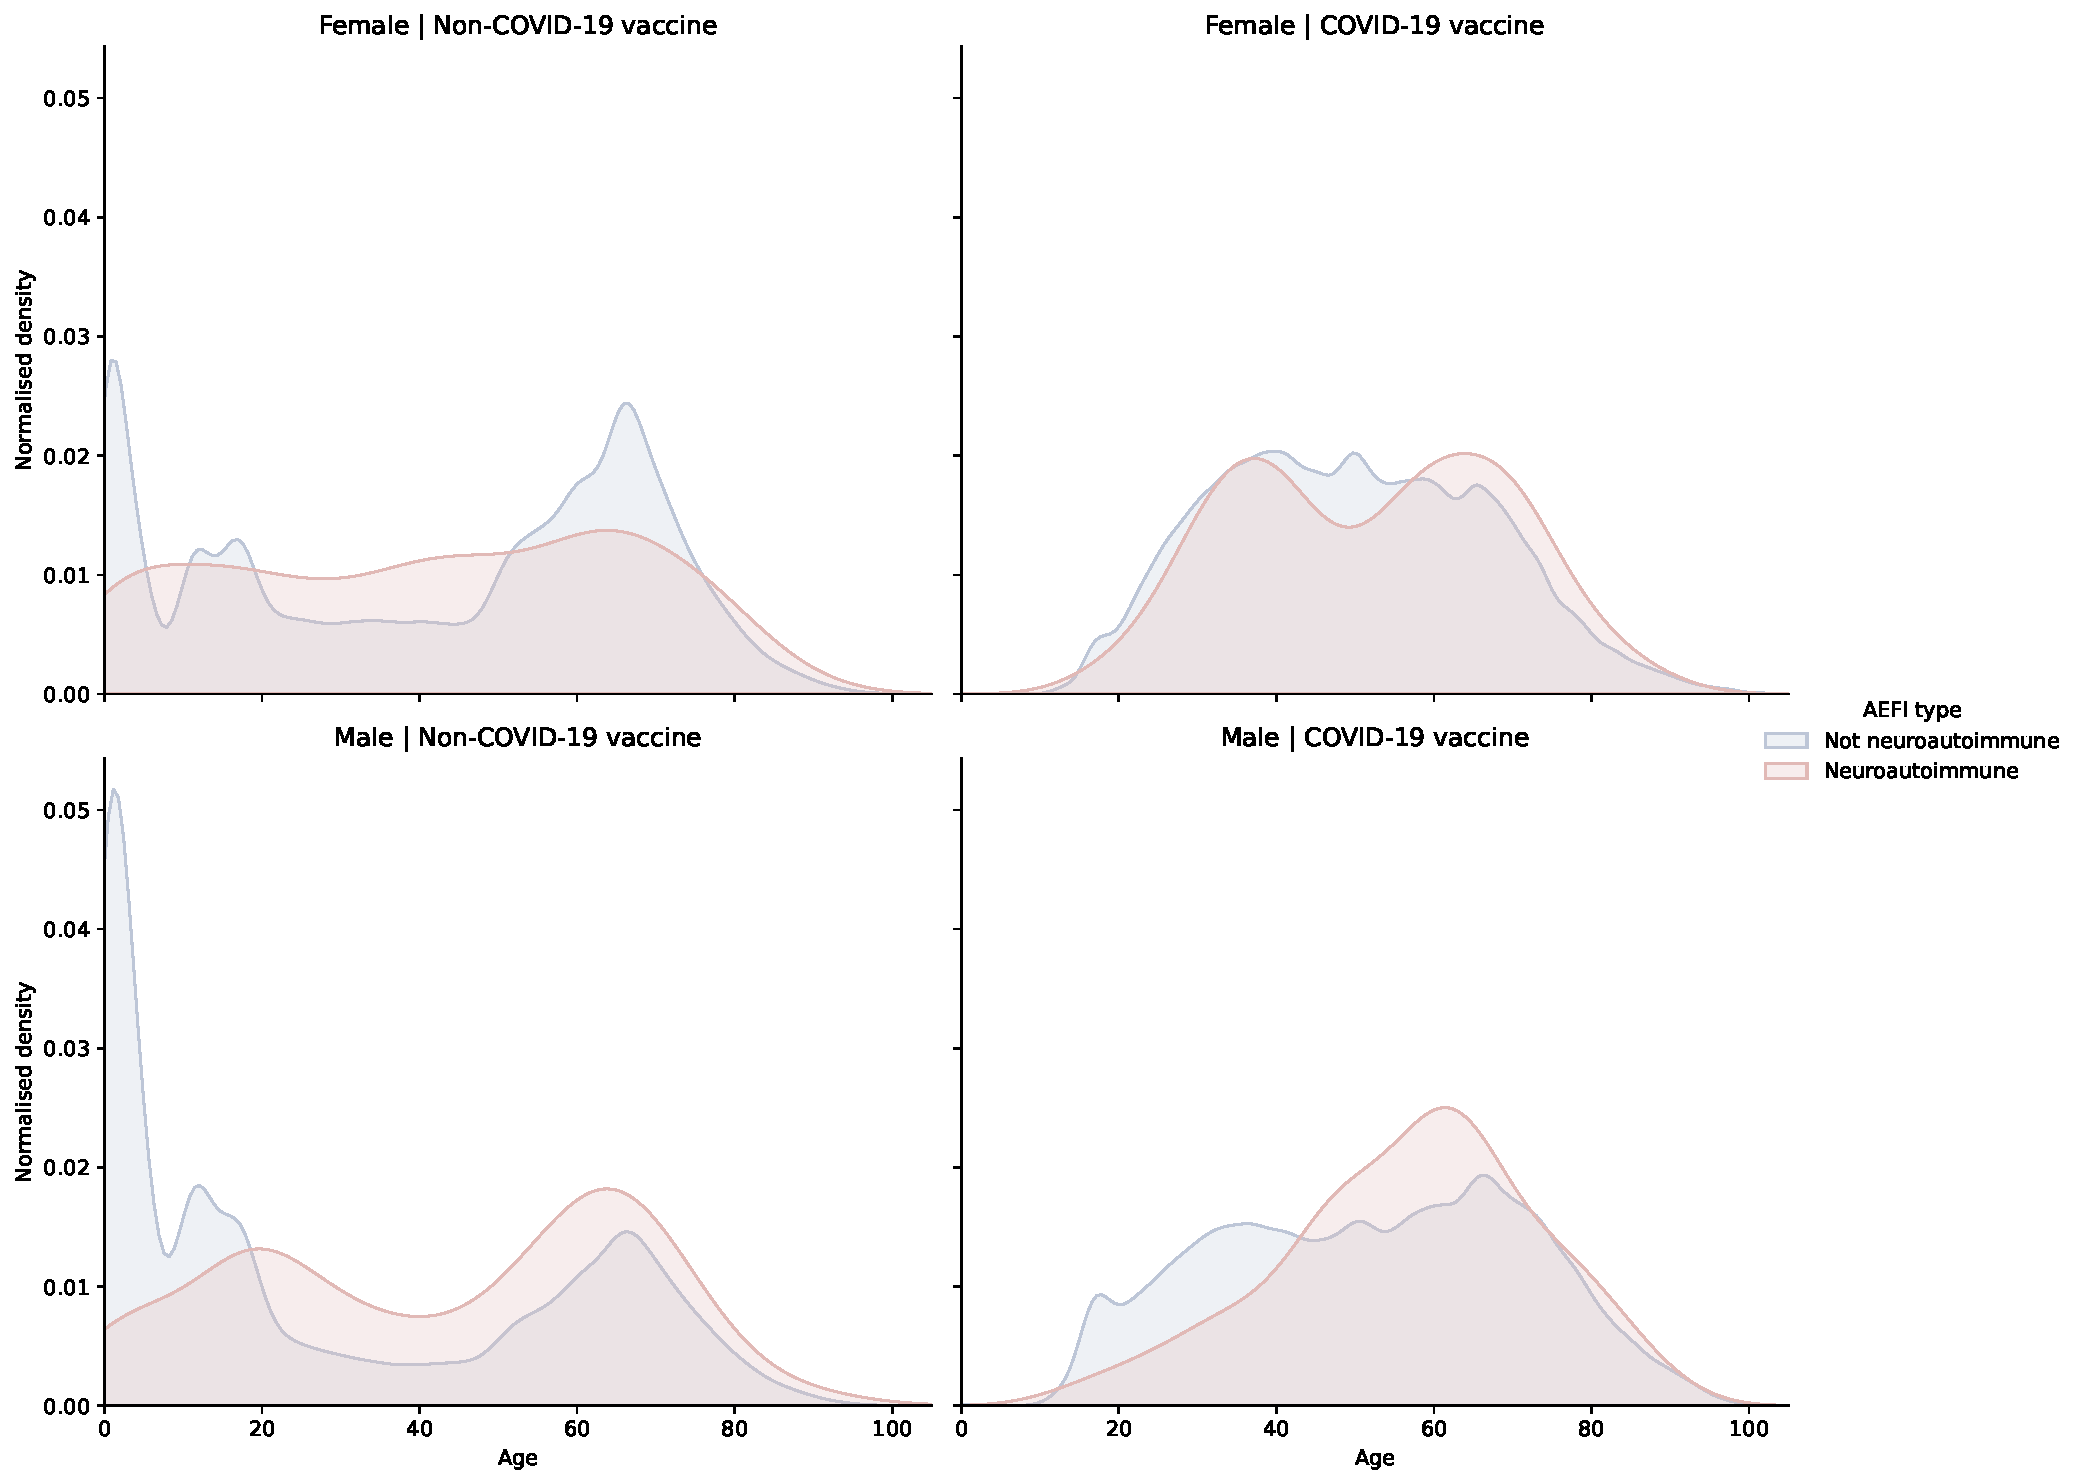
\includegraphics[width=12.5 cm]{age_distribution}
\caption{Distribution of reports by age, partitioned by vaccine type (COVID-19 vs. non-COVID-19 vaccine) and
neuroautoimmune disorder status (neuroautoimmune vs. non-neuroautoimmune symptoms).\label{distribution_by_age}}
\end{figure}

Data was cross-tabulated to yield a 2x2 contingency table for COVID-19 vs. non-COVID-19 vaccines
(Table~\ref{contingency_table}), and the odds ratio was calculated using Fisher's exact test. In addition, a
Pearson's $\chi^2$ test was performed and the Pearson residuals were calculated for each permutation, using
\texttt{statsmodels} v.0.12.2.\cite{seabold2010statsmodels}

\begin{specialtable}[H]
\caption{2x2 contingency table by vaccine type (COVID-19 vs. non-COVID-19 vaccine) and neuroautoimmune
disorder status.\label{contingency_table}}
%%% \tablesize{} %% You can specify the fontsize here, e.g., \tablesize{\footnotesize}. If commented out \small will be used.
\begin{tabular}{ccc}
\toprule
& \textbf{Neuroautoimmune AEFI}	& \textbf{Non-neuroautoimmune AEFI}\\
\midrule
COVID-19 vaccine	    	& 612			    & 1,322,566  \\
Non-COVID-19 vaccine		& 1908              & 1,203,677 \\
\bottomrule
\end{tabular}
\end{specialtable}

Next, symptoms were broken down individually, and a $\chi^2$ distribution fitted. Along with the actual values, the
expected values under the null hypothesis of independence ($H_0$) were ascertained, as well as the Pearson residuals.

Finally, a large contingency table was constructed, calculating the reporting odds ratio of each AEFI for each vaccine
category (VAERS variable \texttt{VAX\_TYPE}), which acts as a superset comprising vaccines that have typically the same
target and same valency (e.g. the Johnson \& Johnson COVID-19 vaccine and the Moderna vaccine are both in the
\texttt{COVID19} vaccine category, whereas a trivalent and a quadrivalent influenza vaccine would be different vaccine
categories due to their difference in valency). For the purposes of constructing this table, a regular expression was
used to filter out a number of entities that are typically recorded in VAERS but which do not indicate an appropriate
denominator for the calculation of the odds ratio. These were used to exclude

\begin{itemize}
    \item normal results (e.g. \texttt{.*(negative|normal)\$}),
    \item mere tests and assays that do not disclose a result (e.g. \texttt{.*assay\$}),
    \item procedures (e.g. \texttt{.*(plasty|insertion|tomy|ery...}),
    \item management of an ongoing medical status or device,
    \item administrative flags (e.g. \texttt{Blood (group|don(or|ation))}), and
    \item COVID-19 related public health interventions (e.g. \texttt{COVID-19 \\ (prophylaxis|immunisation|screening)}).
\end{itemize}

RORs were cross-tabulated by vaccine type and filtered only for symptoms that were categorised as neuroautoimmmune
symptomatic presentations.

%%%%%%%%%%%%%%%%%%%%%%%%%%%%%%%%%%%%%%%%%%
\section{Results}

\subsection{Association with neuroautoimmune AEFIs}

Fisher's two-sided exact test was used to calculate the odds ratio to determine the odds ratio for an association
between reporting a neuroautoimmune AEFI and reporting after/in relationship with a COVID-19 vaccine. This yielded an
OR of 0.292 at $p < 0.0001$ - a statistically highly significant result that indicates COVID-19 vaccination predisposes
to a significantly lower risk – by over 70\% – of reporting a neuroautoimmune side effect rather than any other side
effect. It is important to note that this does not mean that neuroautoimmune side effects are 70\% less frequent, but
rather that the likelihood of reporting a neuroautoimmune side effect over any other side effect is 70\% lower.

\begin{specialtable}[H]
\caption{Pearson residuals by vaccine type (COVID-19 vs. non-COVID-19 vaccine) and neuroautoimmune
disorder status.\label{pearson_residuals}}
%%% \tablesize{} %% You can specify the fontsize here, e.g., \tablesize{\footnotesize}. If commented out \small will be used.
\begin{tabular}{ccc}
\toprule
& \textbf{Neuroautoimmune AEFI}	& \textbf{Non-neuroautoimmune AEFI}\\
\midrule
COVID-19 vaccine	    	& -19.459               & 0.615  \\
Non-COVID-19 vaccine		& 20.386    	        & -0.644 \\
\bottomrule
\end{tabular}
\end{specialtable}

This is confirmed by the Pearson $\chi^2$ residuals that were calculated (see Table~\ref{pearson_residuals}). The residual of neuroautoimmune AEFIs following a COVID-19 vaccine ($-19.459$) indicates that the expected value is significantly higher than the actual value under the assumption of the null hypothesis of independence. It is therefore quite evident that the odds of reporting a neuroautoimmune AEFI over any other AEFI are correlated with whether the preceding vaccine was a COVID-19 vaccine or not, with recipients of COVID-19 vaccines being significantly (70\%) less likely to report a neuroautoimmune AEFI.

\subsection{Association of individual neuroautoimmune AEFIs}

\begin{figure}[H]
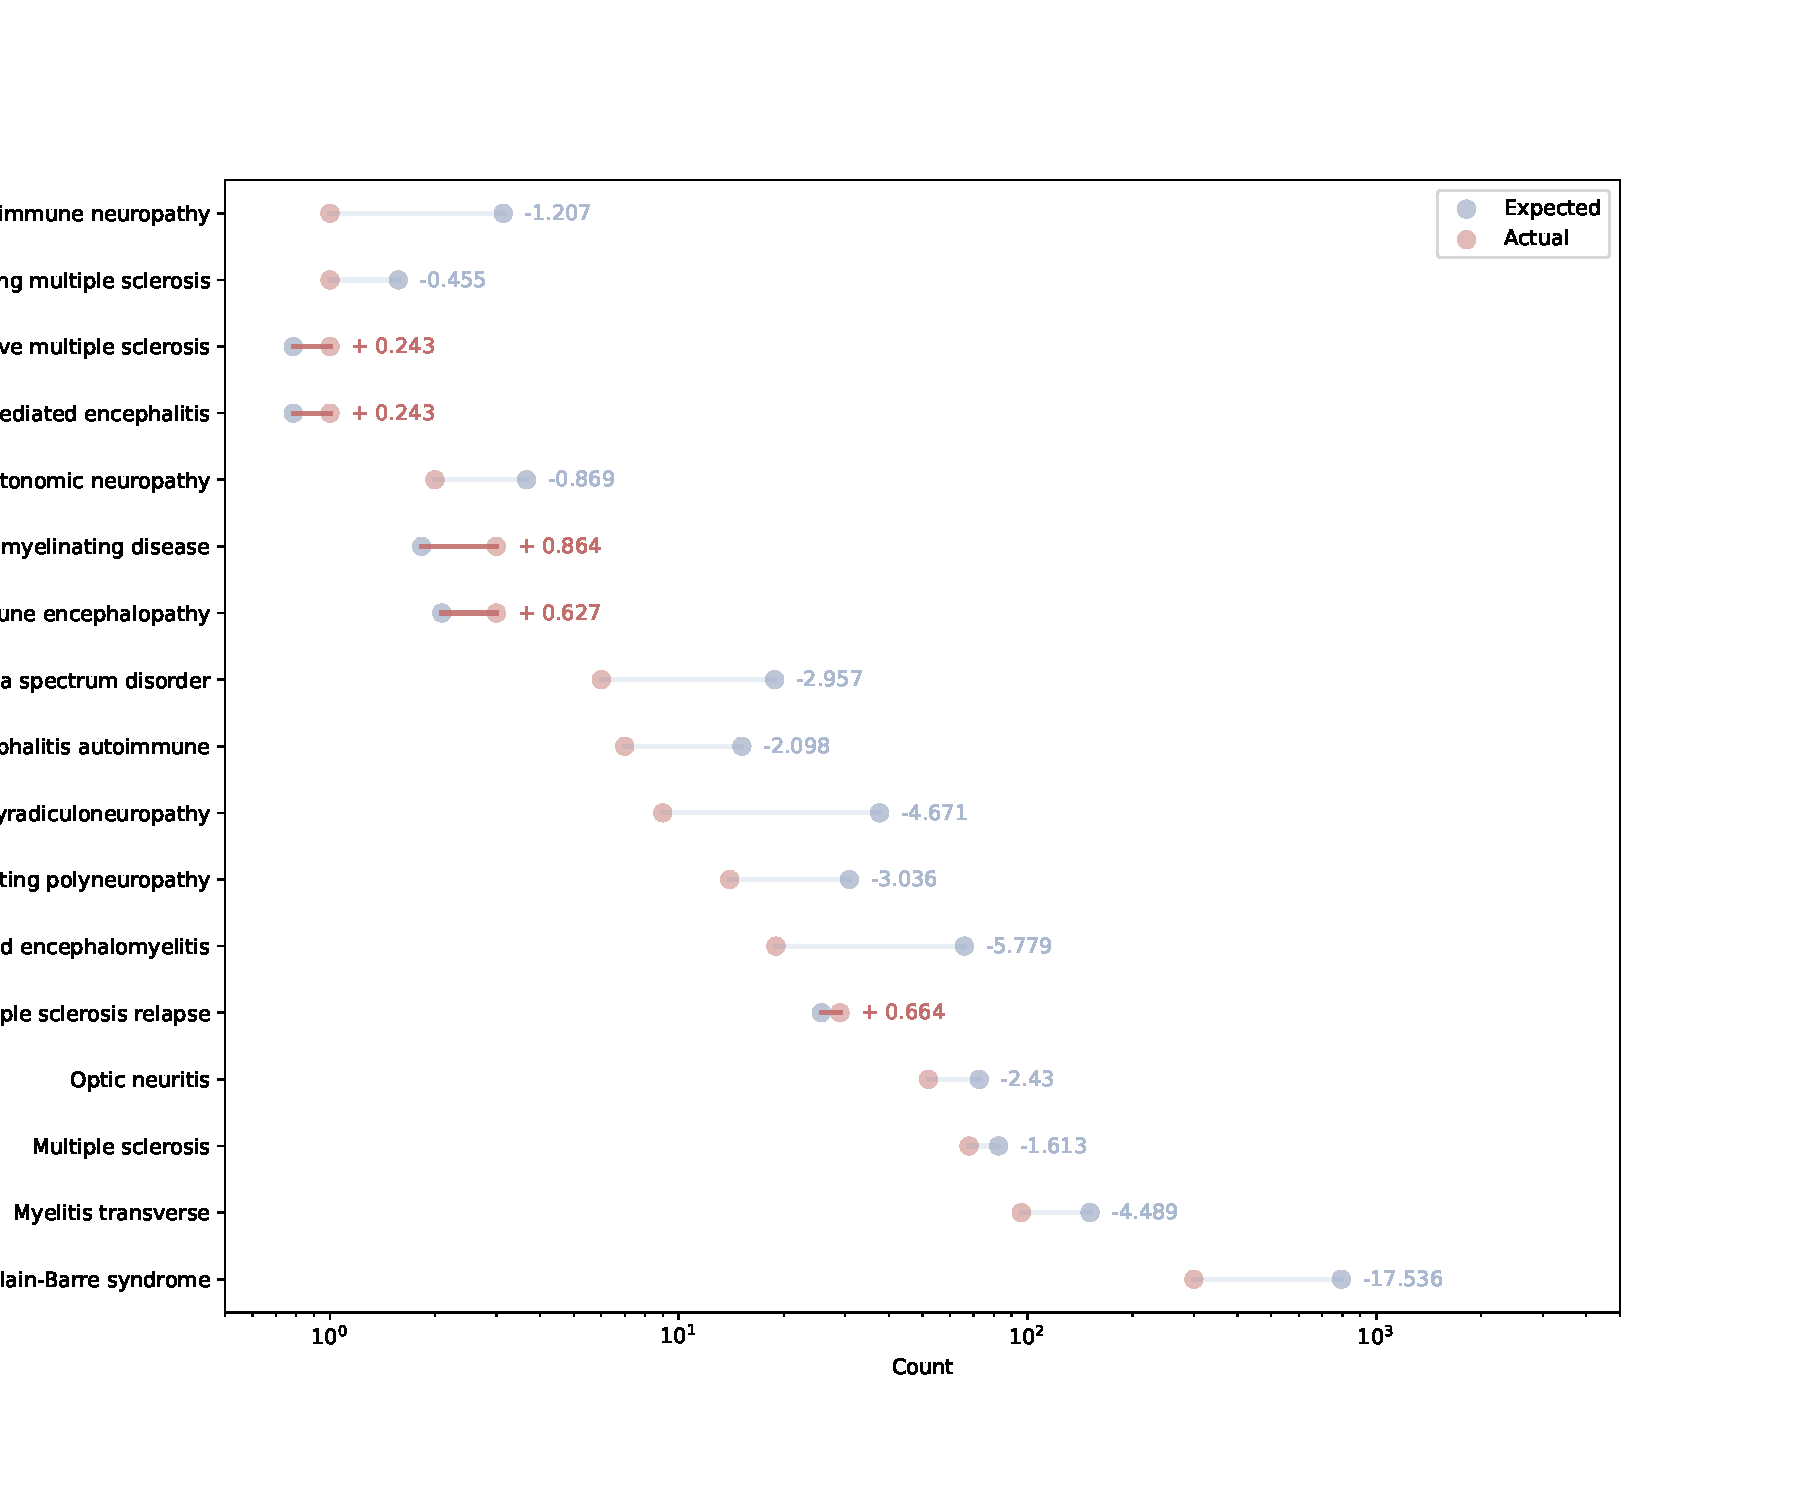
\includegraphics[width=12.5 cm]{expected_vs_actual_by_symptoms}
\caption{Expected vs. actual number of reports for individual neuroautoimmune symptoms based on Pearson's $\chi^2$ test
along with Pearson residuals for COVID-19 vaccines.\label{expected_vs_actual}}
\end{figure}

Following on from these findings, it is not surprising to see that in most cases, the number of actual cases reported
is significantly lower than would be expected under the null hypothesis of independence (see
Figure~\ref{expected_vs_actual}). The notable exceptions are

\begin{itemize}
    \item progressive MS (Pearson residual: 0.243),
    \item immune-mediated encephalitis (Pearson residual: 0.243),
    \item autoimmune demyelinating disease (Pearson residual: 0.864),
    \item autoimmune encephalopathy (Pearson residual: 0.627), and
    \item MS relapse (Pearson residual: 0.664).
\end{itemize}

While the residuals indicate that the deviation is quite small for all of the above, it appears that in contrast with
other vaccines, COVID-19 vaccines appear to result in a relatively higher number than expected of these AEFIs. This
must be considered in the context of actual figures, of course – altogether, these differences account for fewer than
0.25 additional cases of progressive MS and immune-mediated encephalitis, fewer than one case of autoimmune
encephalopathy, fewer than 4 cases of MS relapse and fewer than 1.5 cases of autoimmune demyelinating disease. Of over
1.3m reports, these constitute an excess of six cases, or approx. one in 220,530 reports. Consequently, it remains to
be seen (especially given the low absolute numbers) whether this association remains in evidence as more data accrues,
or, as is more likely, it is part of the noisy undercurrent that is characteristic of passive reporting.

\subsection{Reporting odds ratios between vaccines}

\begin{figure}[H]
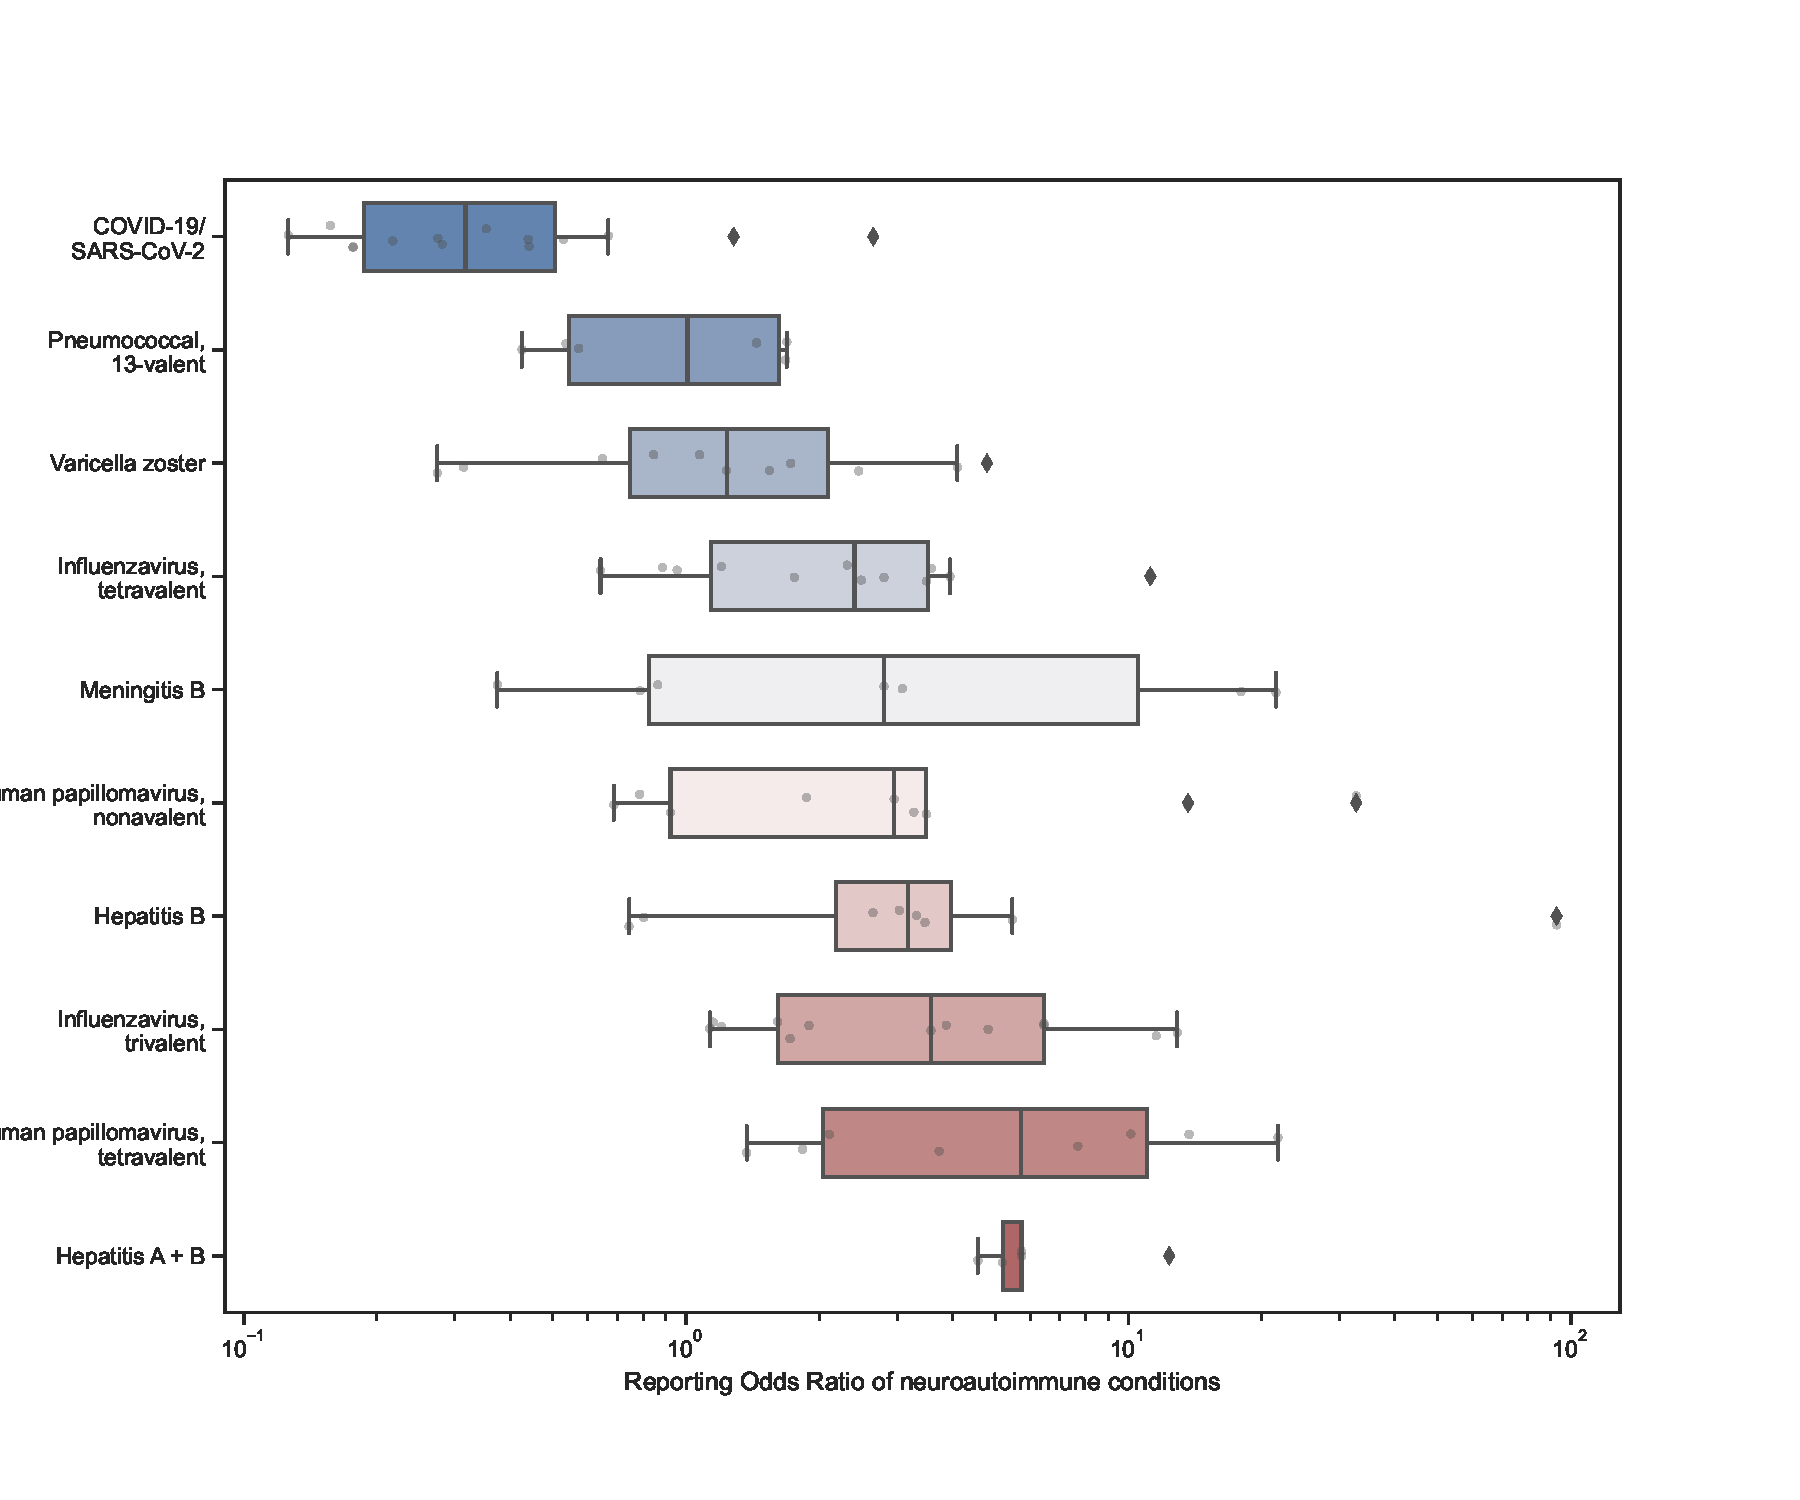
\includegraphics[width=12.5 cm]{ror_by_vaccine_type}
\caption{Reporting Odds Ratios of neuroautoimmune conditions in a range of vaccines approved for adult populations.
\label{ror_by_vaccine_type}}
\end{figure}

As Figure~\ref{ror_by_vaccine_type} shows, the ROR of neuroautoimmune presentations is significantly lower for COVID-19
vaccines than it is for any of the comparator vaccines. The group of comparators was chosen to primarily include
vaccines that have the same age range of approved users to reduce the bias arising from the fact that some vaccines
are typically given in a paediatric context (e.g. MMR), while COVID-19 vaccination was consciously designed to
address older populations first due to their higher overall risk from COVID-19 as well as the relatively higher rate
of respiratory, cardiac and endocrine comorbidities that governed vaccine allocation in the beginning.

%%%%%%%%%%%%%%%%%%%%%%%%%%%%%%%%%%%%%%%%%%
\section{Discussion}

Based on early data from VAERS for reports about COVID-19 vaccinations received on or before 28 May 2021, there
is convincing evidence that COVID-19 vaccines compare remarkably well with other vaccines in respect of
neuroautoimmune AEFIs. Despite the limitations of this study, which drew on passive reporting data with all its
inherent problems, such as reporting bias and the lack of a reliable denominator, we have found evidence that supports
the safety of COVID-19 vaccines with regard to neuroimmunological presentations. Statistical analysis indicated that in
comparison to recipients of other vaccines, those who reported in respect of a COVID-19 vaccines were over 70\% less
likely to report a neuroimmunological presentation than a non-neuroimmunological presentation.

Similarly, the number of reports fell significantly under what was expected in all but two somemwhat cohesive symptom
groups: relapses of MS on one hand and autoimmmune encephalitis on the other. The fact that some forms of autoimmune
encephalitis are distributed bimodally by age with a peak in the third and the seventh decade of life may support a
hypothesis that the increase in cases of autoimmune encephalitis is the consequence of statistical noise and/or
sampling bias due to the higher average age of COVID-19 vaccine recipients in the sample.\cite{shan2021neuronal}
Similarly, multiple sclerosis exhibits a similar bimodality of age distribution, to the point that respective terms
for early-onset (teens to early 30s) and late onset (50s and later) MS have become established in the
literature.\cite{kis2008clinical} Nevertheless, clinicians may, as a matter of abundance of caution, keep a closer eye
on patients with known MS or risk factors for MS (such as previous diagnosis of optic neuritis or CIS/RIS) for signs
of progression or relapse. This may be accompanied by proactively explaining the relative risk of a relapse in the
context of potentially worse clinical outcomes with COVID-19, especially for patients treated with systemic immunosupressants.

Since the start of the global vaccination campaign, evidence has been accumulating for the overall tolerability and
safety of the COVID-19 vaccines. This study seeks to add to our current understanding by quantifying the highly
favourable risk profile of COVID-19 vaccines with regard to neuroautoimmune disorders. While some questions remain open
and conclusions made over early data may have to be reconfirmed through ongoing analysis, the current data supports
the assertion that the COVID-19 vaccine has perhaps the lowest reporting odds ratio for neuroautoimmune disorders of
any vaccine routinely given in adulthood. This is a reassuring indication of safety at a time when concerns about
adverse events still keep most countries from attaining the threshold of collective immunity.

%%%%%%%%%%%%%%%%%%%%%%%%%%%%%%%%%%%%%%%%%%
\vspace{6pt} 

\funding{This research was funded by Starschema Inc. under its intramural research funding programme.}

\dataavailability{VAERS reporting data is available from the CDC's website at \url{https://vaers.hhs.gov}. All code and
scripts supporting this manuscript are deposited at
\url{https://github.com/chrisvoncsefalvay/covid19-neuroautoimmune-aefis} and are made available under the DOI 10.5281/zenodo.4940261.}


\conflictsofinterest{CvC is a consultant to a company that may be affected by the research reported in this paper. The funders had no role in the design of the study; in the collection, analyses, or interpretation of data; in the writing of the manuscript, or in the decision to publish the~results.}


%%%%%%%%%%%%%%%%%%%%%%%%%%%%%%%%%%%%%%%%%%
%% Optional
\abbreviations{Abbreviations}{
The following abbreviations are used in this manuscript:\\

\noindent 
\begin{tabular}{@{}ll}
AEFI 	& 	Adverse event following immmunization 			\\
CDC 	& 	Centers for Disease Control and Prevention 		\\
CIS 	& 	clinically isolated syndrome					\\
EUA 	& 	Emergency Use Authorization						\\
FDA 	& 	Food and Drug Administration					\\
GBS 	& 	Guillain-Barre syndrome							\\
mRNA 	& 	messenger RNA									\\
MS 		& 	multiple sclerosis 								\\
QoL 	& 	quality of life 								\\
RIS 	& 	radiologically isolated syndrome				\\
ROR 	& 	Reporting Odds Ratio							\\
VAERS 	& 	Vaccine Adverse Effect Reporting System			\\
\end{tabular}
}
%%%%%%%%%%%%%%%%%%%%%%%%%%%%%%%%%%%%%%%%%%
\reftitle{References}

\externalbibliography{yes}
\bibliography{bibliography}

\end{document}

